%%%%%%%%%%%%%%%%%%%%%%%%%%%%%%%%%%%%%%%%%%%%%%%%%%%%%%%%%%%%%%%%%%%%%%%%%
%%% PASJ LaTeX template for draft(body)<2014/11/25>
%%% 
%%% IMPORTANT NOTICE FOR AUTHORS
%%% 1. ``\draft'' creates single column and double spaces format.
%%% 2. If you comment out ``\draft'', the output will be double column
%%%    and single space.
%%% 3. For cross-references, the use of \label/\ref/\cite and the 
%%%    thebibliography environment is strongly recommended
%%% 4. Do NOT use \def/\renewcommand.
%%% 5. Do NOT redefine commands provided by PASJ01.cls.
%%% 
%%%%%%%%%%%%%%%%%%%%%%%%%%%%%%%%%%%%%%%%%%%%%%%%%%%%%%%%%%%%%%%%%%%%%%%%%
\documentclass[]{pasj01}
\draft

%\usepackage{graphicx}
%\graphicspath{{figures/}}


\begin{document} 
\Received{}%{yyyy/mm/dd}
\Accepted{}%{yyyy/mm/dd}
%\Published{yyyy/mm/dd}

\title{The bright-star masks for the HSC-SSP survey}

%%% begin:list of authors
% Do NOT capitalize all letters in "textsc".
\author{Jean \textsc{Coupon}\altaffilmark{1}%
%\thanks{jean.coupon@unige.ch}
}
\altaffiltext{1}{Department of Astronomy, University of Geneva, ch. d'\'Ecogia 16, 1290
Versoix, Switzerland}
\email{jean.coupon@unige.ch}

\author{the bright-star mask team\textsc{}\altaffilmark{3}}
%\altaffiltext{3}{}
%\email{ccccc@xxx.xxx.xx.xx}
%%% end:list of authors

%% `\KeyWords{}' always has to be placed before `\maketitle'.
\KeyWords{xxxx: xxxx --- ......} %Do NOT move this preamble from here!

\maketitle

\begin{abstract}
\end{abstract}


\section{Introduction}


The high sensitivity of the Hyper-Suprime-Cam is such that on a typical exposure of a few minutes, point-source objects brighter than $\sim17-19$th magnitude saturate and affect nearby sources. Ideally one would like to directly rely on our catalogue to identify and mask bright stars\footnote{Here, other bright point sources, such as QSOs, are included in the term \emph{bright stars}.}, however, if the pipeline can identify large saturated areas, it is difficult (although not impossible) to precisely measure the required size of masks due to the photometric artefacts caused by the bright stars.  To ease the process, we therefore make use of external data.

A first version of the bright-object masks has been made by Jean Coupon and Nicole Czakon for the S15B and S16A internal data releases, but this version was over conservative in the choice of mask radius and contained about 10\% of bright galaxies, making it non ideal for a number of science cases. The goal here is to update the masks to a much cleaner version (i.e. truly a bright-\emph{star} mask).

In this document we describe the procedure we adopt to automatically construct and validate the bright-star masks for the HSC-SSP broad-band filters $grizY$, using data from the Gaia, Tycho-2, and SDSS surveys. We limit ourselves to the sample of bright stars that saturate on HSC-SSP images (the information on non-saturated stars -- such as brightness and PSF-size -- can be easily gathered HSC-SSP data), that is as complete as possible, and 100\% pure (to avoid masking bright galaxies). We first describe the problem in Section~\ref{sec:pb}, we then describe how we gather a sample of bright stars in Section~\ref{sec:catalogue} and how we construct the masks in Section~\ref{sec:masks}. In a last Section~\ref{sec:valid} we estimate the purity and completeness of the bright stars masks, quantify the improvement on a number of observables, and describe their limitations. We conclude in Section~\ref{sec:conclusions}.



\section{Saturated stars in HSC}
\label{sec:pb}

\subsection{Overview}

The brighter-fatter effect, the diffraction, and electron leaking to nearby pixels, result in (1) isotropic luminous haloes, (2) anisotropic spikes, and (3) unidirectional ``bleed trails'', as shown in Figure~\ref{fig:saturated_star}. The extent of the saturated stars on the image increases with brightness and therefore impact the neighbouring sources through the degradation of the detection performance and the measurements reliability, as well as screening background sources. Here we aim to record the position of such bright stars and to construct photometric masks to reject those unreliable sources.
%

See~Fig\ref{fig:test}

\begin{figure}
 \begin{center}
%  \includegraphics[width=0.49\textwidth]{galfrac.eps}
  \includegraphics[width=80cm]{galfrac.eps}
 \end{center}
 \caption{caption}\label{fig:test}
\end{figure}


%\begin*{figure}
%\center
%  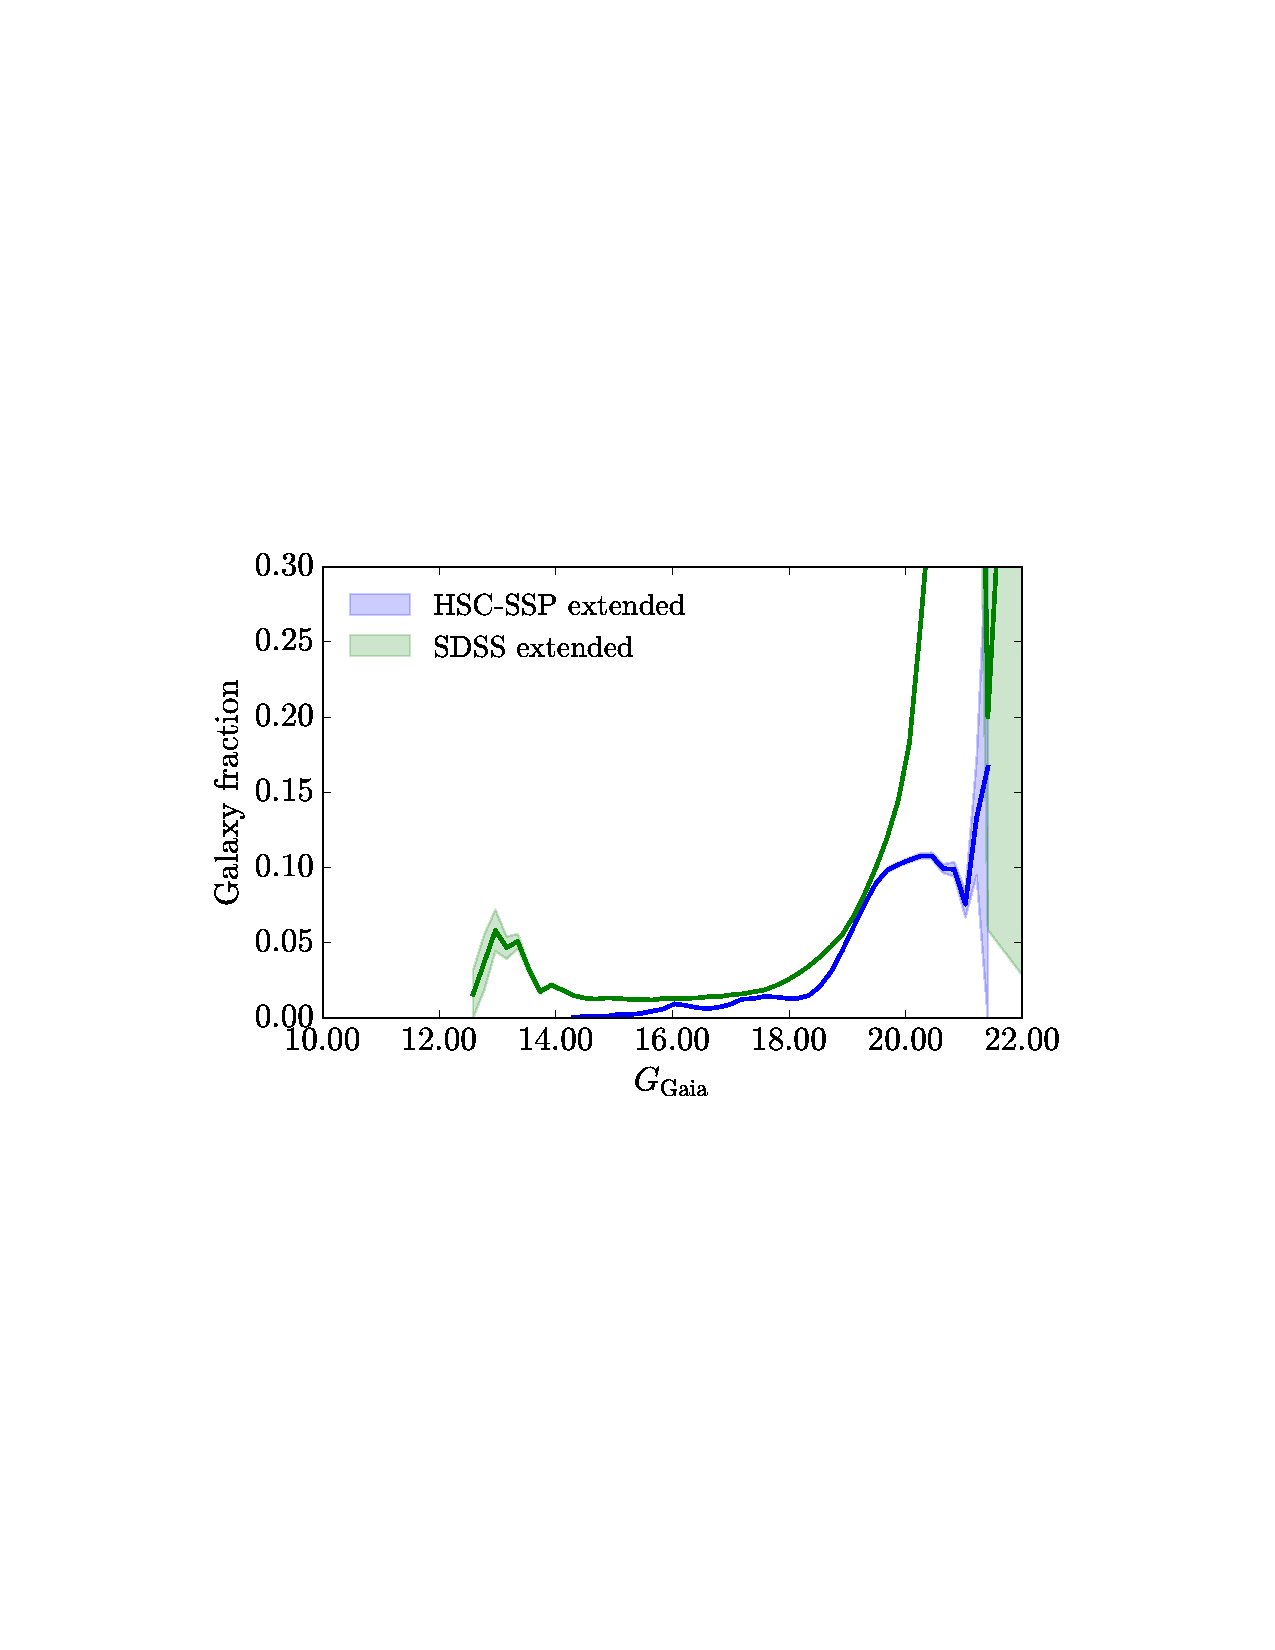
\includegraphics{galfrac.pdf}
%    \caption{An example of a saturated star in HSC-SSP survey in a $i$-band image ($i\sim8$). One can see the horizontal bleed trails, the extended luminous halo and the diffraction patterns.}
%    \label{fig:saturated_star}
%\end*{figure}



\newpage

\section{Section2}

In figure \ref{fig:sample}, ...

%\begin{figure}
 %\begin{center}
 % \includegraphics[width=8cm]{fig1.eps} 
 %\end{center}
%\caption{This is the first figure.}\label{fig:sample}
%\end{figure}


\section{Section 3}

In the theory (\cite{key-1})..........

\subsection{Subsection}

In the theory (\cite{key-2})..........

\subsubsection{Subsubsection}

The resent result from ...........


\newpage

\section{Section 4}

The final ..........


%%%%%%%%%%%%%%%%%%%%%%%%%%%%%%%%%%%%%%%

\begin{table}
  \tbl{This is the first tabular.}{%
  \begin{tabular}{llll}
      \hline
      Name & Value1 & Value2 \\ 
      \hline
      aaa & bbb & ccc & ddd \\
      eee & fff & ggg & hhh \\
      ....\\
      \hline
    \end{tabular}}\label{tab:first}
\begin{tabnote}
This is table note.
\end{tabnote}
\end{table}

\begin{longtable}{cccc}
  \caption{Sample of ``longtable."}\label{tab:LTsample}
  \hline              
  Name & Value1 & Value2 & Value3 \\ 
\endfirsthead
  \hline
  Name & Value1 & Value2 & Value3 \\
\endhead
  \hline
\endfoot
  \hline
\endlastfoot
  \hline
  aaaaa & bbbbb & ccccc & ddddd \\
  ...... & ..... & ..... & ..... \\
  ...... & ..... & ..... & ..... \\
  ...... & ..... & ..... & ..... \\ 
  wwwww & xxxxx & yyyyy & zzzzz \\
\end{longtable}

%%%%%%%%%%%%%%%%%%%%%%%%%%%%%%%%%%%%%%%


\begin{ack}
Acknowledgement should be placed at end of main text.
(NOT after the Appendix.)
\end{ack}


\appendix 
\section*{Case of single paragraph}

\section{Case of two or paragraphs}

\section{Case of two or paragraphs}


%%%
% See the manual for the detail.
%%%
\begin{thebibliography}{}
% Journals(e.g. A\&A,ApJ,AJ,NMRAS,PASP ...)
% Authors, Year, Journal, Vol#, Page#
% Journal Title Abbreviation >> http://www.asj.or.jp/pasj/Jabb.html
\bibitem[Aauthor et al.(2001)]{key-1}
  Aauthor, A., Bauthor, B., Cauthor, C.\ 2001, PASJ, vol, page
\bibitem[Aauthor \& Bauthor(2003a)]{key-2}
  Aauthor, A., \& Bauthor, B.\ 2003a, PASJ, vol, page   
\bibitem[Aauthor \& Bauthor(2003b)]{key-3}
  Aauthor, A., \& Bauthor, B.\ 2003b, PASJ, vol, page  
\bibitem[Aauthor, Cauthor, and Dauthor(2000)]{key-3}
  Aauthor, A., Cauthor, C., \& Dauthor, D.\ 2000, PASJ, vol, page   
% Books
\bibitem[Aauthor \& Eauthor(2003b)]{key-3}
  Aauthor, A., \& Euthor, E.\ 2003b, Name of Book (Tokyo: Publisher) ch.0    
% Editorial Books
\bibitem[Dauthor(2001)]{key-n}
  Dauthor A.~A.\ 2001, in Name of Book,
   ed.\  D.~Editor (Tokyo: Publisher), page
\end{thebibliography}


\end{document}
